\let\negmedspace\undefined
\let\negthickspace\undefined
\documentclass[journal]{IEEEtran}
\usepackage[a5paper, margin=10mm, onecolumn]{geometry}
%\usepackage{lmodern} % Ensure lmodern is loaded for pdflatex
\usepackage{tfrupee} % Include tfrupee package

\setlength{\headheight}{1cm} % Set the height of the header box
\setlength{\headsep}{0mm}  % Set the distance between the header box and the top of the text

\usepackage{gvv-book}
\usepackage{gvv}
\usepackage{cite}
\usepackage{amsmath,amssymb,amsfonts,amsthm}
\usepackage{algorithmic}
\usepackage{graphicx}
\usepackage{textcomp}
\usepackage{xcolor}
\usepackage{txfonts}
\usepackage{listings}
\usepackage{enumitem}
\usepackage{mathtools}
\usepackage{gensymb}
\usepackage{comment}
\usepackage[breaklinks=true]{hyperref}
\usepackage{tkz-euclide} 
\usepackage{listings}
% \usepackage{gvv}                                        
\def\inputGnumericTable{}                                 
\usepackage[latin1]{inputenc}                                
\usepackage{color}                                            
\usepackage{array}                                            
\usepackage{longtable}                                       
\usepackage{calc}                                             
\usepackage{multirow}                                         
\usepackage{hhline}                                           
\usepackage{ifthen}                                           
\usepackage{lscape}
\begin{document}

\bibliographystyle{IEEEtran}
\vspace{3cm}

\title{1.8.14}
\author{EE24BTECH11016 - Dhwanith M Doddahundi}

% \maketitle
% \newpage
% \bigskip
{\let\newpage\relax\maketitle}

\renewcommand{\thefigure}{\theenumi}
\renewcommand{\thetable}{\theenumi}
\setlength{\intextsep}{10pt} % Space between text and floats




\textbf{Question: }\\
The distance of the point $\vec P\brak{-6, 8}$ from the origin is\\
\solution { 
\begin{table}[h!]    
  \centering
  \begin{tabular}{c|c}
    \hline
    \textbf{Species} & \textbf{Concentration(milli equivalent/L)}\\
    \hline
    Chloride$(Cl^{-})$ & 15\\
    Sulphate$(SO_{4}^{2-}$ & 15 \\
    Carbonate$(CO_{3}^{2-}$ & 05 \\
    BiCarbonate$(HC0_{3}^{-}$ & 30 \\
    Calcium$(Ca^{2+})$ & 12 \\
    Magnesium$(Mg^{2+})$ & 18 \\ 
    pH & 8.5 \\
    \hline
    \end{tabular}

  \caption{Input parameters}
  \label{tab1.1.9.2}
\end{table}
\begin{align}
	d&=\norm{\vec P-\vec O}\\
 \implies d&=\sqrt{\brak{\vec P-\vec O}^\top\brak{\vec P-\vec O}}\\
 \implies d&=\sqrt{\myvec{-6\\8}\myvec{-6&8}}\\
 \implies d&=\sqrt{\brak{-6}^2+8^2}\\
 \implies d&=\sqrt{100}\\
 \implies d&=10
    \end{align}
   The distance of the point $\vec P\brak{-6,8}$ from the origin is 10 units.
\begin{figure}[!ht]
    \centering
	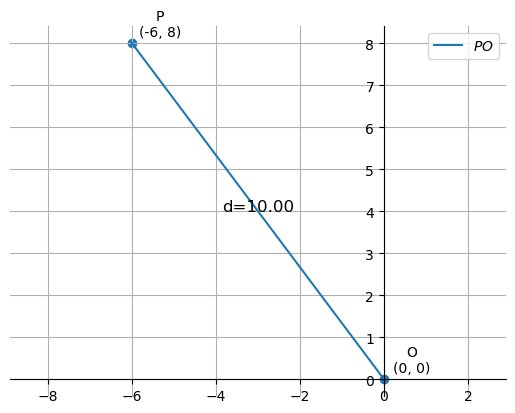
\includegraphics[width=1\textwidth]{plots/plot.png}
    \caption{Distance between points $P$ and $O$}
    \label{fig:plot}
\end{figure}  
   }
\end{document}
